%%%%%%%%%%%%%%%%%%%%%%%%%%%%%%%%%%%%%%%%%%%%%%%%%%%%%%%%
%%%%%%%%%%%%%%%%%%%%%%%%%%%%%%%%%%%%%%%%%%%%%%%%%%%%%%%%
\section[MC]{Monte-Carlo event simulation}
\setcounter{tocdepth}{2}

\begin{frame}
\begin{center}
Monte-Carlo event simulation
\end{center}
\end{frame}

\subsection{Monte-Carlo simulations}
\begin{frame}{Monte-Carlo simulations}
\vspace{-.2cm}
\begin{block}{Central concepts}
\scriptsize \centering{ Usage of random variables and large samplings to calculate mathematical quantities in complex configurations.}\\
In particle physics (referred to LHC) $\to$ Simulation of collisions at three levels:
\begin{itemize}
\item Partonic level: Scattering of partons inside protons.
\item Hadronic level: Showering and hadronization of collision products.
\item Detector level: Simulation of the detector response to the particles generated in a collision.
\end{itemize}
\end{block}

\begin{figure}[!Hhtbp]
  \begin{center}
    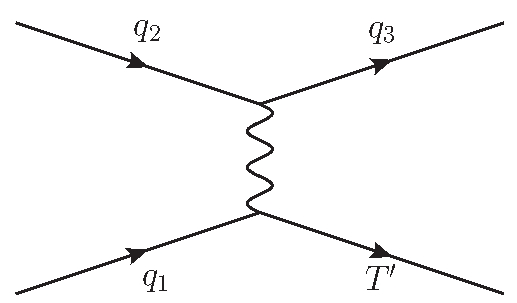
\includegraphics[width=0.3\textwidth]{../figs/Tchannel_T_single.jpg}
    \includegraphics[width=0.35\textwidth]{Hadronization.png}
    \includegraphics[width=0.3\textwidth]{detector_part.png}
  \end{center}
\end{figure}

\end{frame}


\begin{frame}{Parton simulation}
\vspace{-.2cm}

\begin{columns}
\begin{column}{.50\textwidth}
  \begin{block}{}\tiny
    \begin{itemize}
    \item Model proposed to understand collisions of non-fundamental particles.
    \item Valence quarks of a proton are the $u$ and $d$
    \item Sea: $b$, $c$ or $s$ quarks and gluons
    \item Parton distribution function: $f\equiv f(x,Q^{2})$ is the number density of a given quark or gluon as a function of the resolution scale $Q^{2}$ and the fraction of momentum carried by the parton $x$
    \item Simulation done up to a perturbative level: Tree-level or Leading order (LO), one loop or Next-to-Leading-Order (NLO), two loops or Next-to-Next-to-Leading-Order (NNLO), ...
    \end{itemize}
  \end{block}
\vspace{-.3cm}
\begin{block}{}\tiny
\textbf{Tool}: MadGraph $\to$ Matrix-element generator for event generation, calculation of LO cross sections and particle widths. This tool is specially interesting for implementations of BSM models.
\end{block}
\vspace{-.3cm}
\begin{block}{}\tiny
\textbf{Figure}: Martin-Stirling-Thorne-Watt proton PDF for $Q^{2}= 10\, \text{GeV}^{2}$ [left] and $Q^{2}= 10^{4}\, \text{GeV}^{2}$ [right]. $x$ is the fraction of momentum carried by the parton and $f(x,Q^{2})$ the PDF function.
\end{block}
\vspace{-.3cm}
\begin{block}{}\tiny
\textbf{Equation}: $f_{i,j}$ corresponds to the PDF's of the initial partons, $\mathcal{M}_{ij\rightarrow lm}$ is the matrix element of the process
\end{block}
\end{column}

\begin{column}{.50\textwidth}
\begin{figure}[!Hhtbp]
  \begin{center}
    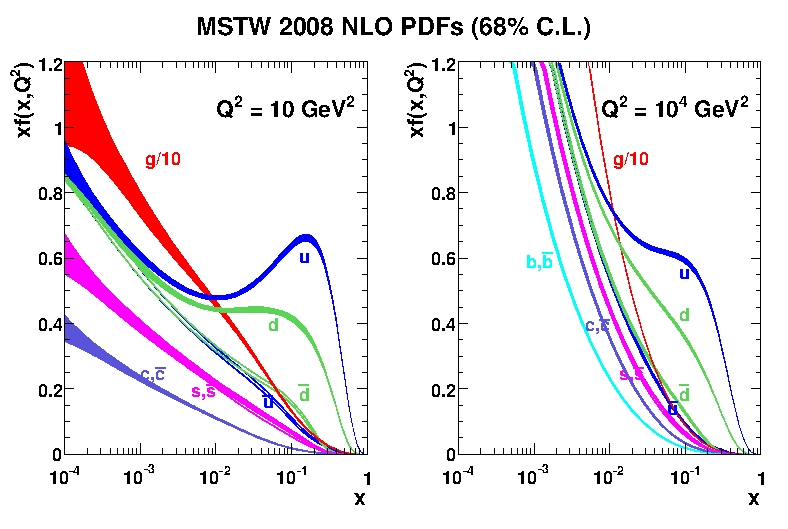
\includegraphics[width=1.0\textwidth]{../figs/mstw2008nlo68cl_allpdfs.jpg}
    %\caption{Martin-Stirling-Thorne-Watt proton PDF for $Q^{2}= 10\, \text{GeV}^{2}$ [left] and $Q^{2}= 10^{4}\, \text{GeV}^{2}$ [right]. $x$ is the fraction of momentum carried by the parton and $f(x,Q^{2})$ the PDF function.}
    %\label{fig:MSTW}
  \end{center}
\end{figure}
\vspace{-.2cm}
{\tiny
\begin{eqnarray}
  %\label{eq:DiffXS}
d\sigma_{ij\rightarrow lm} & = & \left( \int_{0}^{1}\int_{0}^{1}f_{i}(x_{i},Q^{2})f_{j}(x_{j},Q^{2})dx_{i}dx_{j} \right) \nonumber \\
  & \times & \frac{d^{3}p_{l}}{(2\pi)^{2}2E_{l}}\frac{d^{3}p_{m}}{(2\pi)^{2}2E_{m}} \nonumber \\
  & \times & \delta^{4}\left( p_{i}+p_{j}-p_{l}-p_{m} \right) \nonumber \\
  & \times & |\mathcal{M}_{ij\rightarrow lm}|^{2} \nonumber                                     
\end{eqnarray}
}%

\end{column}

\end{columns}
\end{frame}


\begin{frame}{Hadron and Detector simulation}
\vspace{-.2cm}

\begin{columns}
\begin{column}{.50\textwidth}
  \begin{block}{Hadron simulation}\scriptsize
    \begin{itemize}
    \item Quarks produced from hard interaction $\to$ not seen freely due to strong interaction.
    \item Two processes simulations:
      \begin{itemize}\scriptsize
      \item Showering: radiation from initial or final states.
      \item Hadronization: formation of hadrons from final state quarks and gluons.
      \end{itemize}
    \item Hadronization simulation generates the ``soft'' part of the event. Parton simulation generates the hard (interaction) part.
    \end{itemize}
  \end{block}
\vspace{-.3cm}
\begin{block}{}\tiny
\textbf{Tool}: Pythia $\to$ it could take the events produced by a matrix-element generator. If it hadronizes partonic level events, a special procedure (merging) for the interface between the two generations must be done to assure ``physical'' simulations. If not, it generates directly the hadrons from the hard interaction.
\end{block}
\end{column}

\begin{column}{.50\textwidth}
  \begin{block}{Detector simulation}\scriptsize
    \begin{itemize}
    \item Simulation of the detector response to particles simulated in the collision (after hadronization).
    \item Detailed simulation of the detector: subdetectors, cells, layers, electronic cards, ...
    \item It is done as close as possible to reality, however some real detector problems. Two possibilities to solve remaining issues:
      \begin{itemize}\scriptsize
      \item Generate run-dependent MC simulations
      \item Apply corrections to generic MC simulations, to get closer to data.
      \end{itemize}
    \end{itemize}
  \end{block}
\vspace{-.3cm}
\begin{block}{}\tiny
\textbf{Tool}: GEANT 4 $\to$ CMS private detector simulation, with all details of the detector. DELPHES $\to$ Tool to simulate a generic detector with the main pieces: tracking system embedded in a magnetic field, calorimeters and muon system.
\end{block}

\end{column}

\end{columns}
\end{frame}


\begin{frame}{Interface between partonic and hadronic steps}
\vspace{-.2cm}

\begin{columns}
\begin{column}{.50\textwidth}
  \vspace{-.2cm}
  \begin{block}{Merging - MLM procedure}\scriptsize
    Procedure to grant a correct matching between ME and PS:
    \begin{itemize}
    \item ME generation, partons with a minimal $k_{T}$ distance $Q^{X}_{cut}$.
    \item Jet reconstruction from partons with $k_{T}$ algorithm $\to$ n-jets (n-partons)
    \item PS from partons, with a minimal $k_{T}$ distance $Q_{cut}$ (Merging scale)
    \item Jet reconstruction from hadrons with $k_{T}$ algorithm $\to$ N-jets.
    \item Match jets to partons.
    \item Discard events if N>n or not all partons were matched to jets. 
    \end{itemize}
    The correctness of the matching is determined by the choice of $Q^{X}_{cut}$ and $Q_{cut}$.
  \end{block}
\end{column}

\begin{column}{.50\textwidth}
\begin{figure}[!Hhtbp]
  \begin{center}
    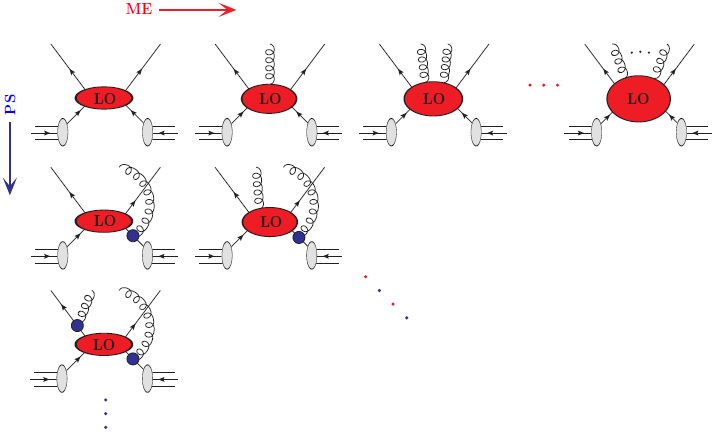
\includegraphics[width=1.1\textwidth]{../figs/PSMEInterface.png}
    %\caption{ME and PS contributions to events with several partons in the final state in a leading order MC simulation.}
    %\label{fig:PSME}
  \end{center}
\end{figure}
  \vspace{-.4cm}
  \begin{block}{}\scriptsize
    \begin{itemize}
    \item Matrix-Element: hard interaction processes (left to right)
    \item Parton shower: soft radiation processes (up to bottom)
    \item When adding additional jets to a process, a possible overlap between ME and PS can occur.
    \end{itemize}
  \end{block}
\end{column}

\end{columns}
\end{frame}

\begin{frame}{Optimizing the merging procedure}
\vspace{-.2cm}
\begin{columns}
\begin{column}{.50\textwidth}
  \begin{block}{}\tiny
    The optimal values of $Q^{X}_{cut}$ and $Q_{cut}$ depend of:
    \begin{itemize}
    \item The process 
    \item Kinematic cuts
    \item Center of mass energy
    \end{itemize}
  \end{block}
\end{column}
\begin{column}{.50\textwidth}
  \begin{block}{}\tiny
    To study the correctness of the choice:
    \begin{itemize}
    \item DJR diagrams
    \item Transition between $n$ and $n-1$ jet multiplicities as a function of the merging scale
    \end{itemize}
  \end{block}
\end{column}
\end{columns}

\vspace{-.2cm}
\begin{figure}[!Hhtbp]
  \begin{center}
    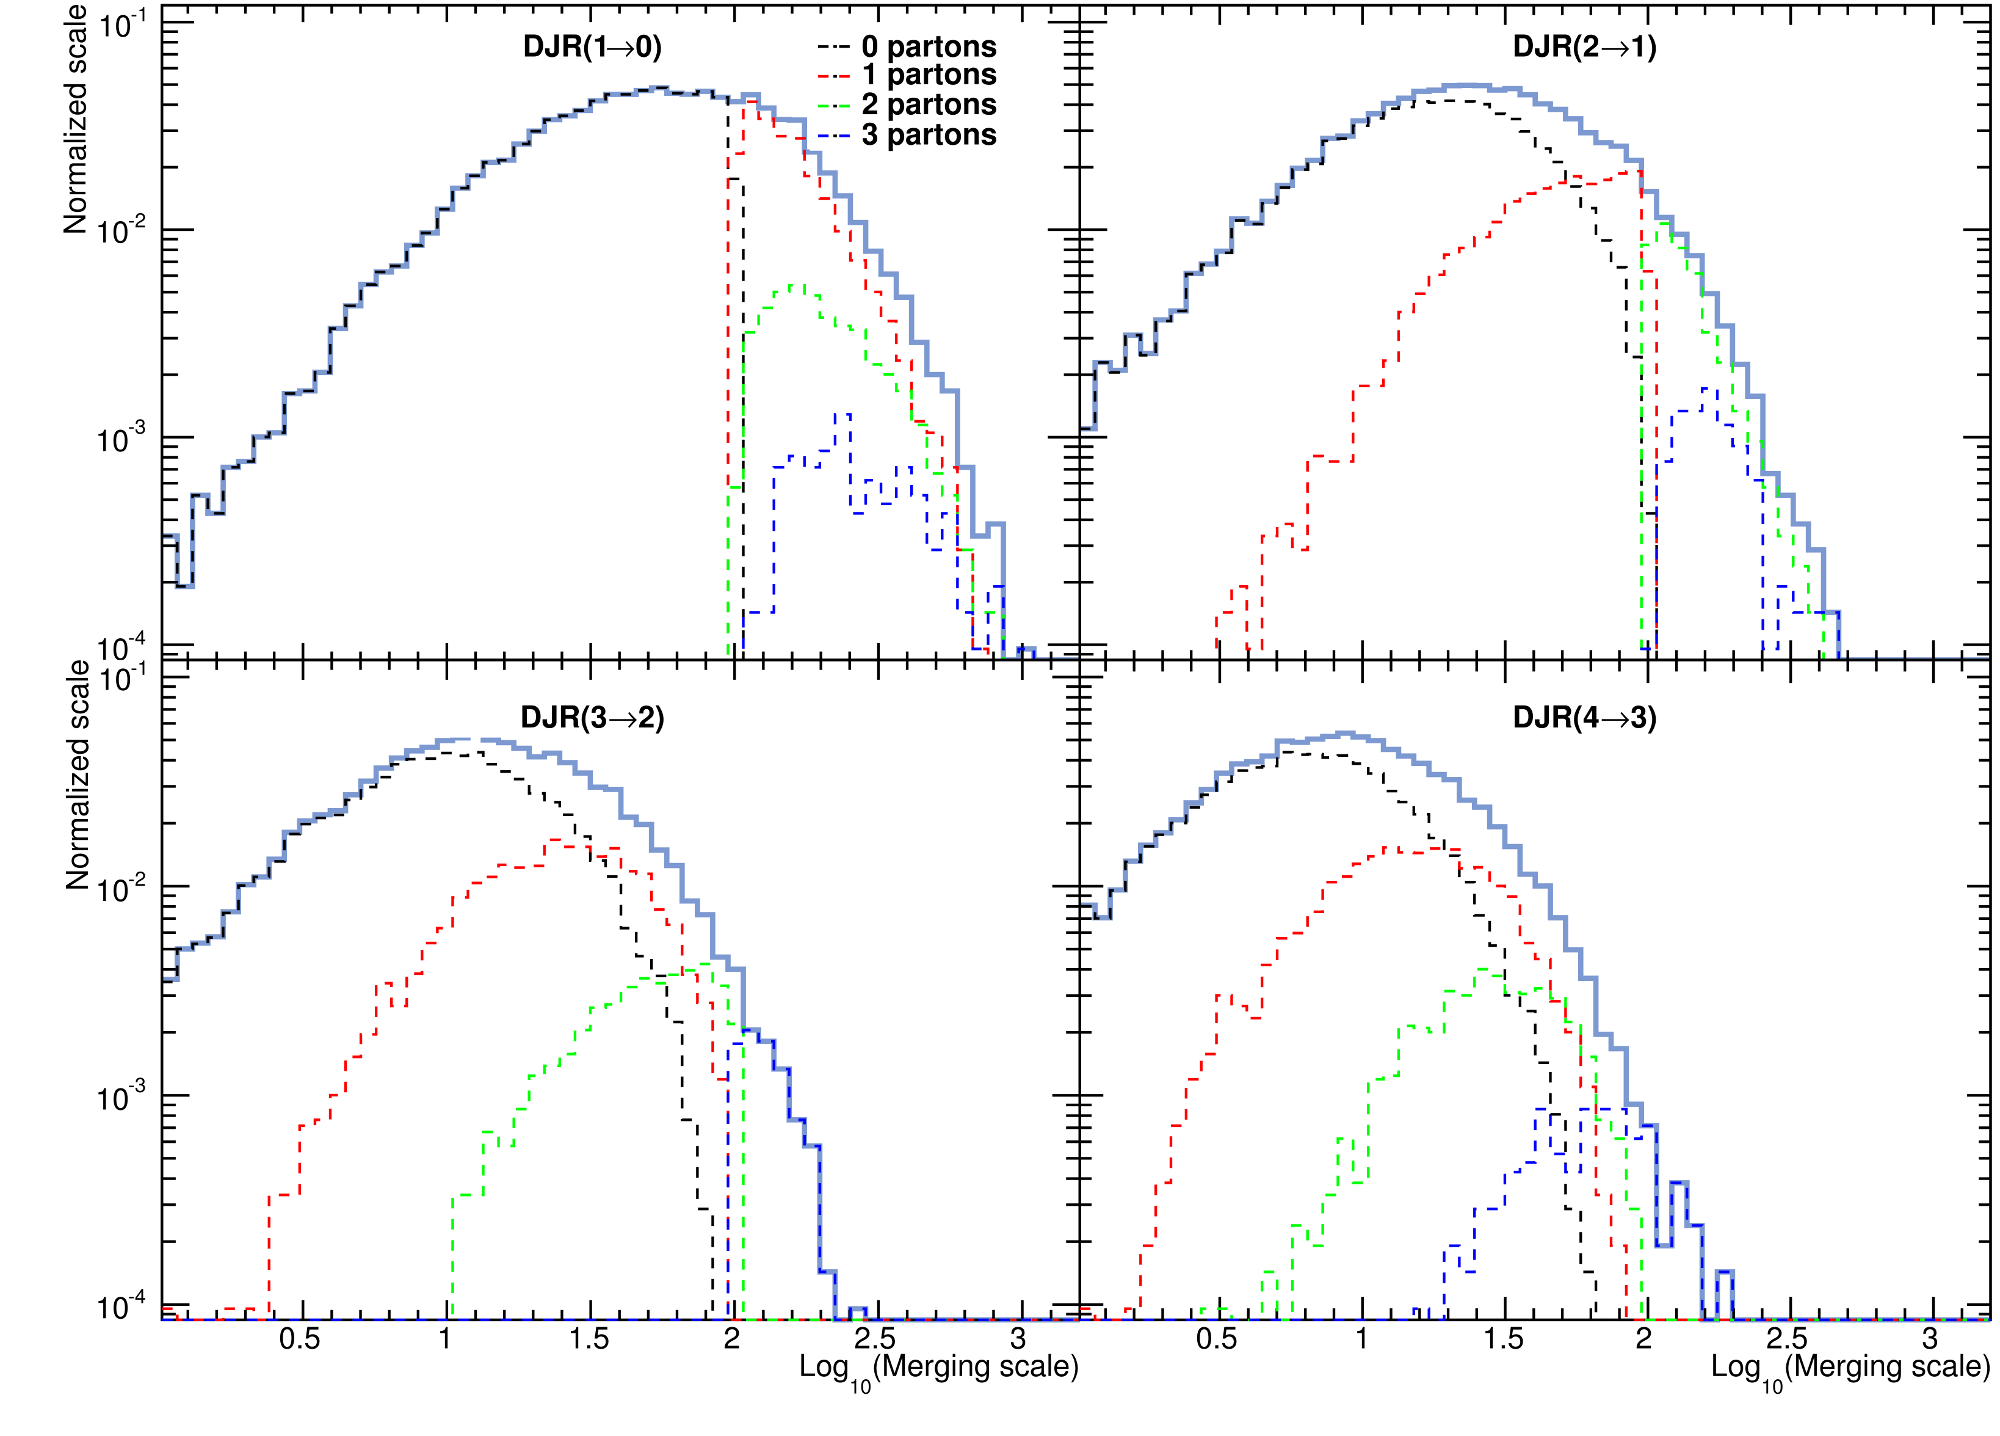
\includegraphics[width=0.5\textwidth]{../figs/DJR_q100_xq20_TTJets13TeV.png}
    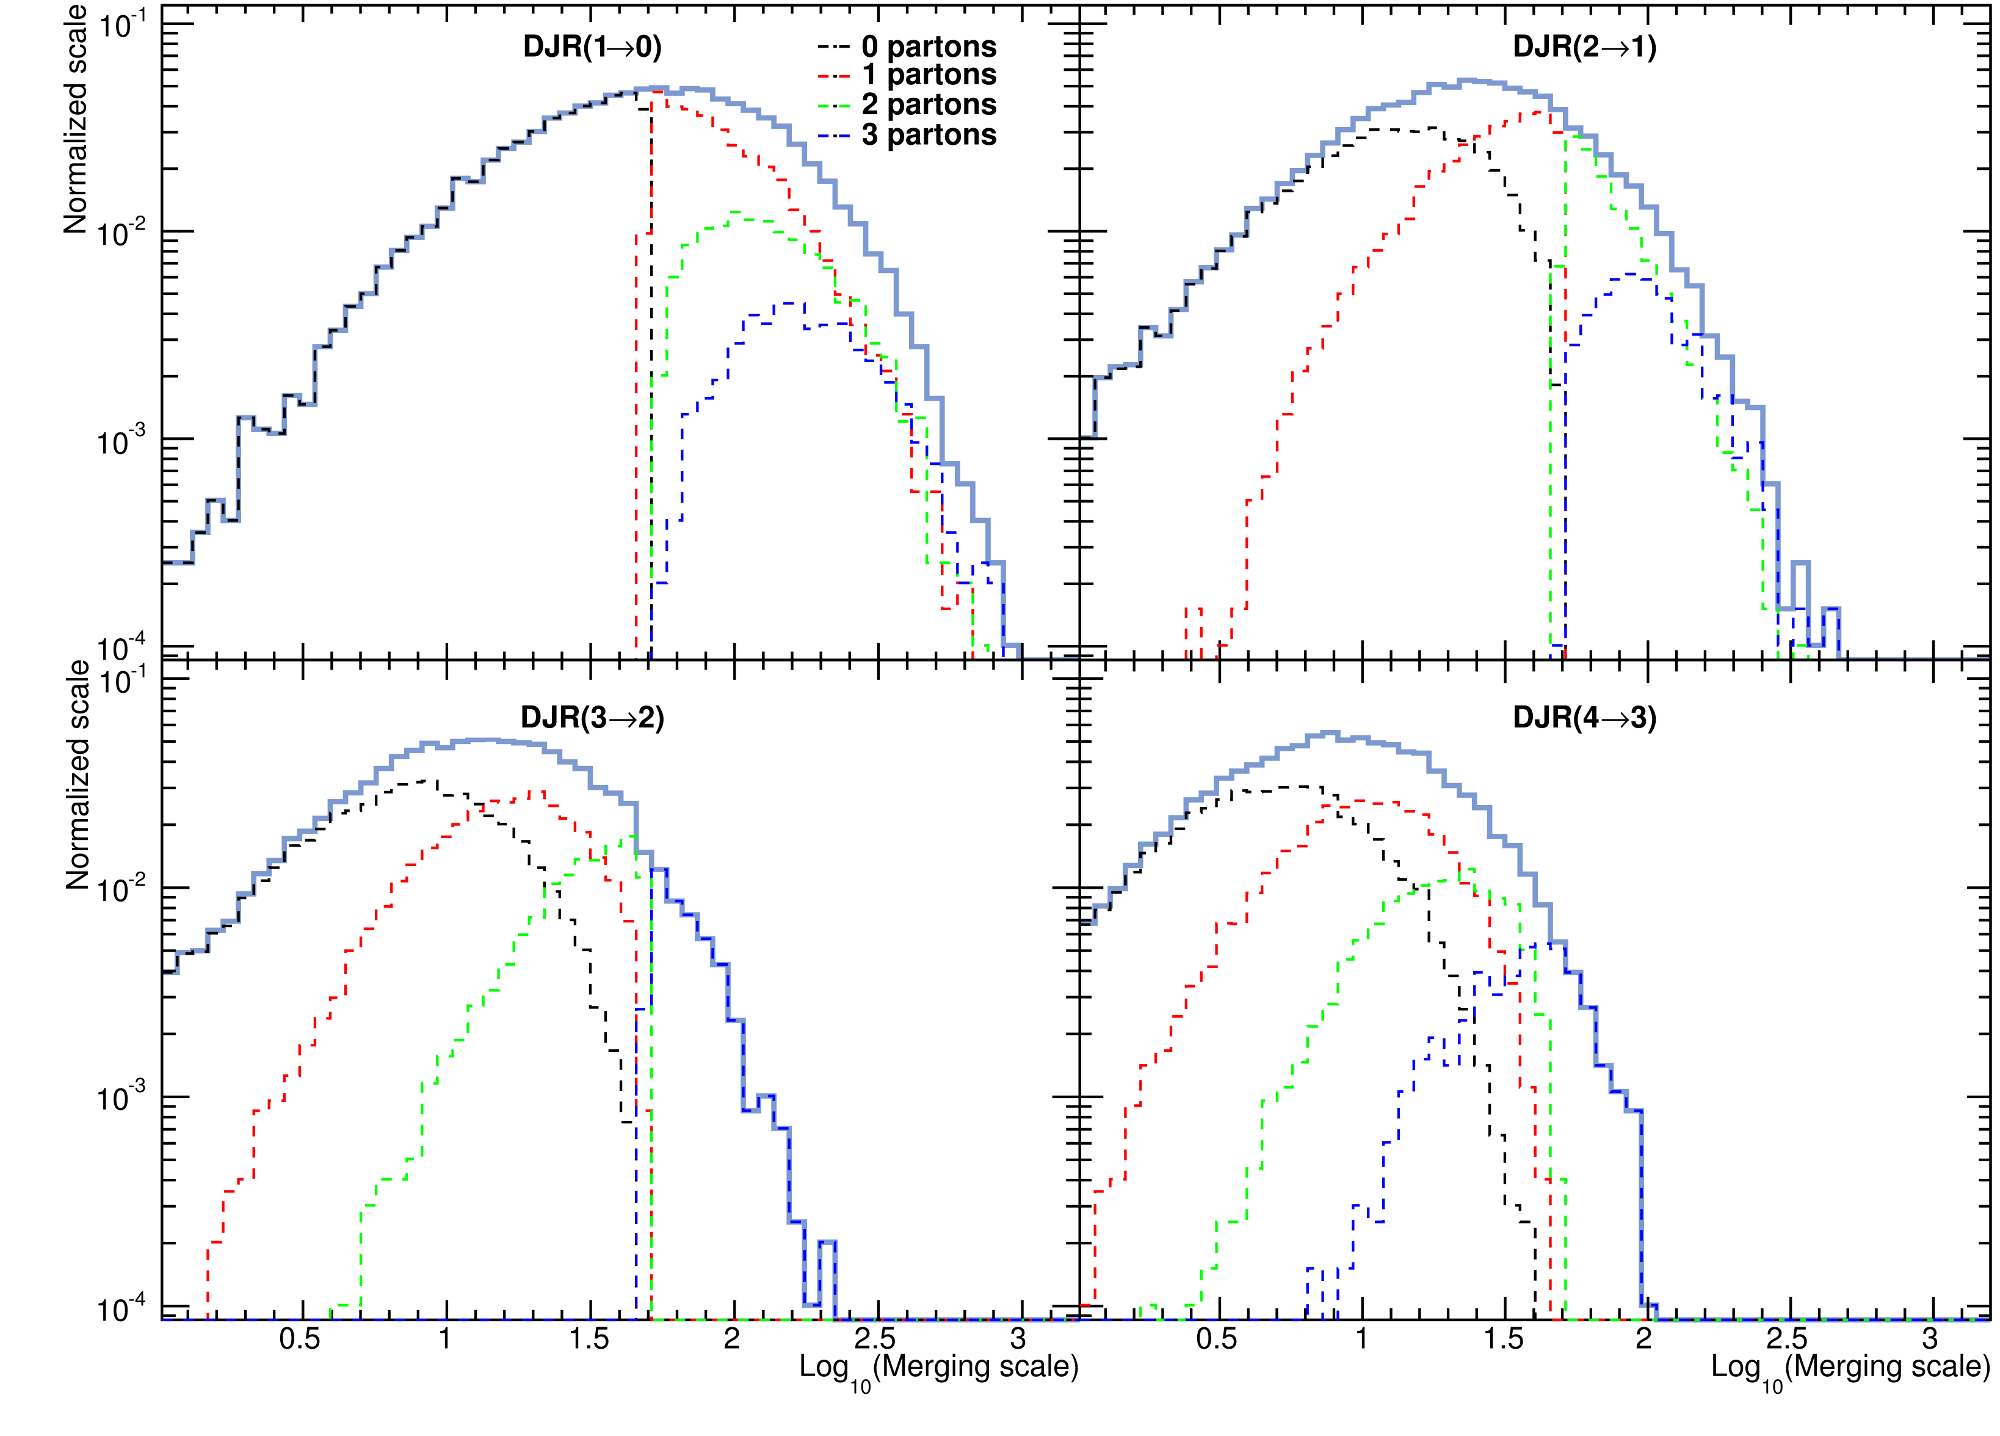
\includegraphics[width=0.5\textwidth]{../figs/DJR_q50_xq20_TTJets13TeV.png}
    %\caption{DJR diagrams for 13 TeV top pair production with $Q_{cut}=100$ GeV and $Q^{X}_{cut}=20$ GeV [optimal case] (top) and $Q_{cut}=60$ GeV and $Q^{X}_{cut}=20$ [non-optimal] (bottom). Bottom figure shows a discontinuity in the transition from 3 to 2 partons at the point where blue-dashed and green-dashed curves meet.}
    %\label{fig:TTJetsMerging}
  \end{center}
\end{figure}

\vspace{-.2cm}
  \begin{block}{}\tiny
    \textbf{Figure}: DJR diagrams for 13 TeV top pair production with $Q_{cut}=100$ GeV and $Q^{X}_{cut}=20$ GeV [optimal case] (left) and $Q_{cut}=60$ GeV and $Q^{X}_{cut}=20$ [non-optimal] (right). Right figure shows a discontinuity in the transition from 3 to 2 partons at the point where blue-dashed and green-dashed curves meet.
  \end{block}

\end{frame}

\begin{frame}{Validation studies on MadGraph}
\vspace{-.4cm}
\begin{columns}
\begin{column}{.50\textwidth}
  \begin{block}{Release validation}\tiny
    New releases are validated against old ones, for different processes.\\
    \textbf{Figure}: Comparison between 1.4.8 (MGOldV) and 1.5.11 (MGLatestV) MadGraph releases for SM \Z+jets production with \Z~decaying into neutrinos. $p_{T}$ of jets [top], $\eta$ of jets [bottom].
  \end{block}
\vspace{-.5cm}
\begin{figure}[!Hhtbp]
  \begin{center}
    %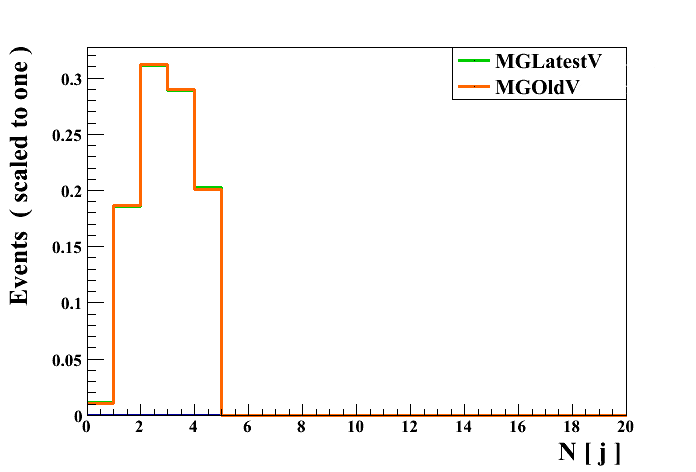
\includegraphics[width=0.45\textwidth]{../figs/ZjetsRelVal0.png}
    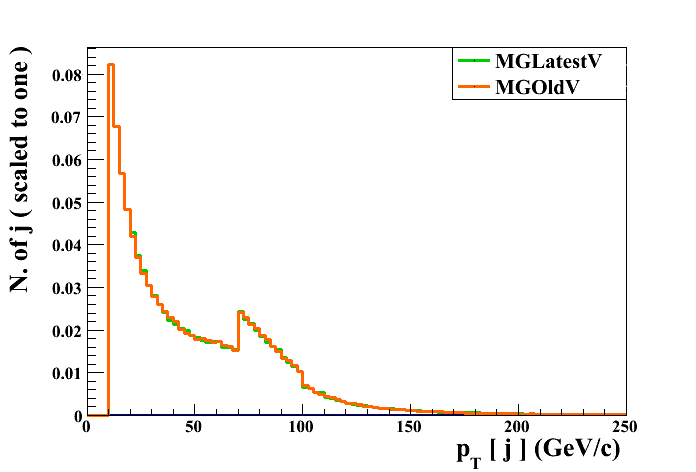
\includegraphics[width=0.75\textwidth]{../figs/ZjetsRelVal1.png}\\
    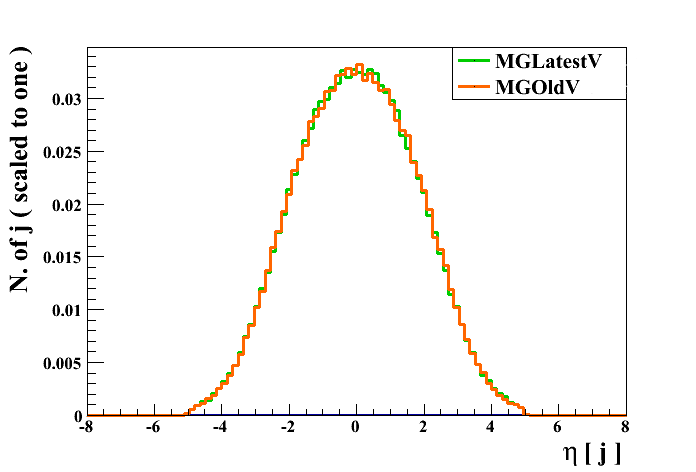
\includegraphics[width=0.75\textwidth]{../figs/ZjetsRelVal2.png}
    %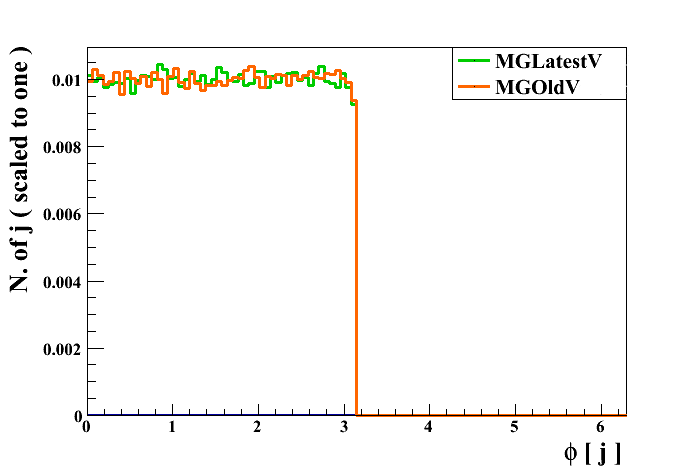
\includegraphics[width=0.45\textwidth]{../figs/ZjetsRelVal3.png}
    %\caption{Comparison between 1.4.8 (MGOldV) and 1.5.11 (MGLatestV) MadGraph releases for SM \Z+jets production with \Z~decaying into neutrinos. Number of jets [left-up], $p_{T}$ of jets [right-up], $\eta$ of jets [left-down] and $\phi$ of jets [right-down]. As expected, no deviation is observed.}
    %\label{fig:ZRelVal1}
  \end{center}
\end{figure}
\end{column}

\begin{column}{.50\textwidth}
  \begin{block}{RIVET toolkit}\tiny
    Comparison of different generators with real data \\
    \textbf{Figure}: \W~boson $p_{T}$ measured by ATLAS experiment in muon final states compared to different MC simulations. py6 stands for Pythia 6, py8 for Pythia 8, MGpy6 MadGraph interfaced with Pythia 6 and PWG for Powheg. MadGraph with Pythia 6 gives the best description of experimental data.
  \end{block}
  \begin{figure}[!Hhtbp]
  \begin{center}
    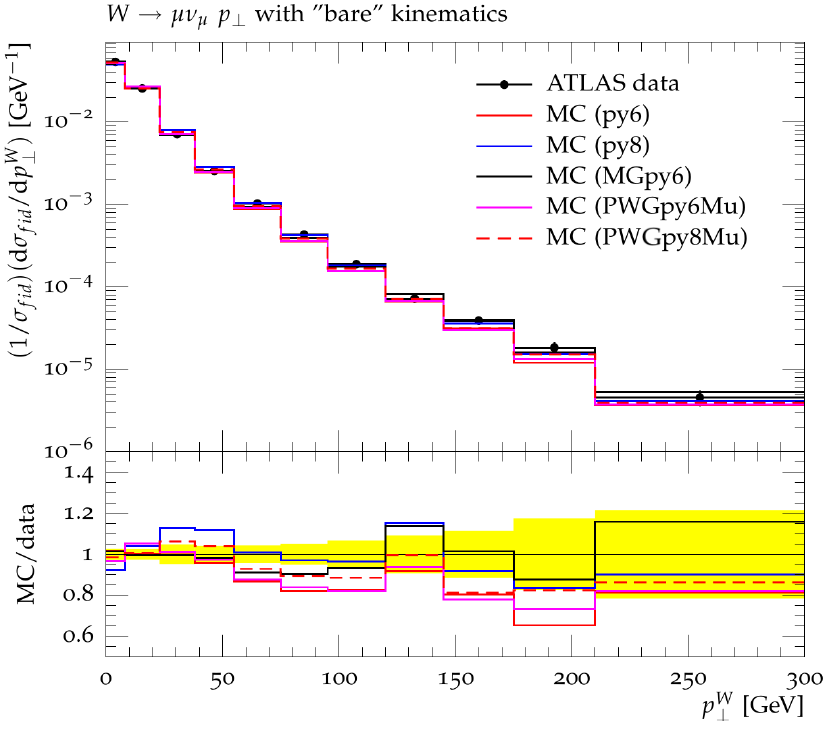
\includegraphics[width=1.0\textwidth]{../figs/Wpt_rivet.png}
    %\caption{\W~boson $p_{T}$ measured by ATLAS experiment in muon final states compared to different MC simulations. py6 stands for Pythia 6, py8 for Pythia 8, MGpy6 MadGraph interfaced with Pythia 6 and PWG for Powheg. MadGraph with Pythia 6 gives the best description of experimental data.}
    %\label{fig:WVal}
  \end{center}
\end{figure}
\end{column}
\end{columns}

\end{frame}